% !TEX spellcheck = en_US

% !TEX root = elastophi-report.tex


\section{Partition of the matrix in admissible blocks}
\label{section:partition}

In the sequel, for any subsets $t,s\subset \llbr1,3N\rrbr$, let $\mA_{t,s}$ refer to a $3N \times 3N$ matrix with coefficients equal to zero, except for the sub-block obtained from $\mA$ 
by restricting indices to the set $t\times s$. 
%We define $\mA_{b}$ similarly for any $b\subset \llbr 1,3N\rrbr\times \llbr 1,3N\rrbr$.

\bigskip
Two important conclusions should be drawn from the discussion of the previous paragraph. The first 
conclusion is that, due to the singularity of the integral kernel, the singular values of the matrix given 
by (\ref{GalerkinMatrix}) do \textit{not} decrease exponentially i.e.~this matrix is not admissible. 
As a consequence, the ACA compression strategy of Section \ref{sec:LowRankApprox} is not directly applicable 
to this matrix. 

\bigskip
However sub-blocks of the matrix $\mA$ given by (\ref{GalerkinMatrix}) may be admissible (i.e.~have exponentially 
decreasing singular values). To build an approximation of $\mA$ allowing a substantial reduction of the cost of 
matrix-vector products, it would be sufficient to find a sparse matrix $\mA_{\mrm{sp}}\in \C^{3N\times 3N}$ such that 
\begin{align}
\mA = \mA_{\mrm{sp}} + \sum_{t\times s\in \mathscr{B}} \mA_{t,s}
\label{eq:decomposition}
\end{align}
where $\mathscr{B}$ is a subset of $\llbr 1,3N\rrbr\times \llbr 1,3N\rrbr$, and each 
$\mA_{b}$ is admissible. Indeed with such a decomposition, one may consider $\mA' = \mA_{\mrm{sp}} + \sum_{t\times s\in \mathscr{B}} \mA_{b}'$
as a good approximation for $\mA$, where each $\mA_{b}'$ is obtained from $\mA_{b}$ after application of the ACA compression 
procedure described in Section \ref{sec:LowRankApprox}. 

%In this manner, keeping $\mathcal{O}(1)$ terms (i.e.~a few terms) from each 
%ACA compression procedure the cost of a matrix-vector product is now $\mathcal{O}(N\log N)$.


\bigskip
The second conclusion that can be drawn from the discussion of Section \ref{sec:GalerkinMatrix} is that the Galerkin discretization establishes 
a correspondence between the numbering of unknowns on the one end, and some spatial distribution of degrees of freedom. This gives an insight 
on how to find admissible (and thus compressible) sub-blocks inside the matrix $\mA$ as described in the following.

\quad\\
For a ball $\mB_{s}\subset \R^{3}$, define $s = \{j \in\llbr 1,3N\rrbr\;\vert \;\mrm{supp}(\bpsi_{j})\subset \mB_{s}\}$. 
For another ball $\mB_{t}\subset \R^{3}$, define $t\subset \llbr1,3N\rrbr$ accordingly.  
The more $\mB_{s}$ and $\mB_{t}$ are far from each other, the faster the singular values of $\mA_{t,s}$ will decrease because the Green kernel, and so the interaction, will be more regular (see Remark \ref{remark:err_decrease} for an example).

The distance between $\mB_{t}$ and $\mB_{s}$ that may be considered as sufficient for the admissibility of $\mA_{t, s}$ depends on the radius of these balls. 
Such a criterion shall be referred later on as \textit{admissibility criterion}. Current literature provides various 
admissibility criterion. It should be considered as problem dependent. For the project Elasto$\Phi$, we considered the 
following admissibility criterion (see \cite{Rjasanow2007})
\begin{equation}\label{AdmissibilityCondition}
\mrm{min}\big( \mrm{diam}(\mB_{t}),\mrm{diam}(\mB_{s})\big)< \eta\;\mrm{dist}(\mrm{B}_{t},\mrm{B}_{s}),
\end{equation}
where $\eta>0$ is a fitting parameter. For the present problem, the typical values of $\eta$ that we considered  
range from $\eta = 0.1$ to $\eta = 10$. 

The decomposition (\ref{eq:decomposition}) relies on the admissible blocks, so that we need to find them in an efficient way. To do so, we build cluster trees, that is to say, we organize the set of geometric elements as a binary tree such that each node of the tree is a cluster of geometric points. The two sons of a cluster/node are obtained by doing a balanced decomposition. In practice, we compute the center of the cluster and then we do a principal component analysis (PCA), so that we can cut in half the cluster with an hyperplane orthogonal to the first principal component (which is the direction of maximal extension) and containing the center. Examples of the first four levels of such cluster trees are given in Figures \ref{fig:cluster_tree_fractures} and \ref{fig:cluster_tree_faults}.

\begin{figure}
\centering
\subfloat[][Initial mesh.]
   {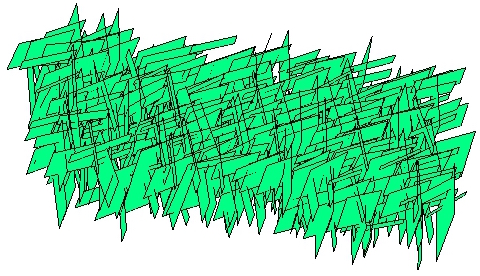
\includegraphics[width=.4\textwidth]{../images/visu_maillage450Fracsbis.jpg}} \quad
\subfloat[][Cluster at the first level.]
   {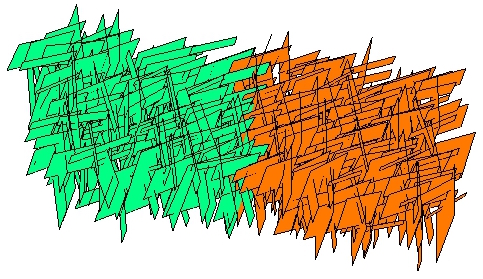
\includegraphics[width=.4\textwidth]{../images/VisuPartmaillage450Fracsdepth1.jpg}} \\
\subfloat[][Cluster at the second level.]
   {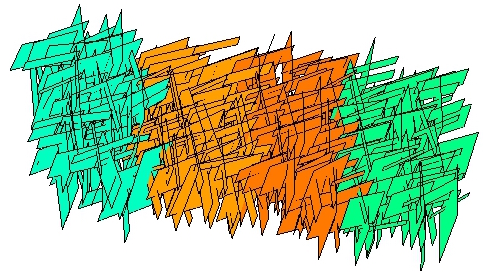
\includegraphics[width=.4\textwidth]{../images/VisuPartmaillage450Fracsdepth2.jpg}}  \quad
\subfloat[][Cluster at the third level.]
   {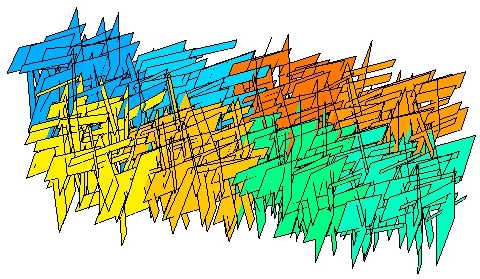
\includegraphics[width=.4\textwidth]{../images/VisuPartmaillage450Fracsdepth3.jpg}} \\
\caption{Cluster tree for a discrete fracture network (DFN).}
\label{fig:cluster_tree_fractures}
\end{figure}

\begin{figure}
\centering
\subfloat[][Initial mesh.]
   {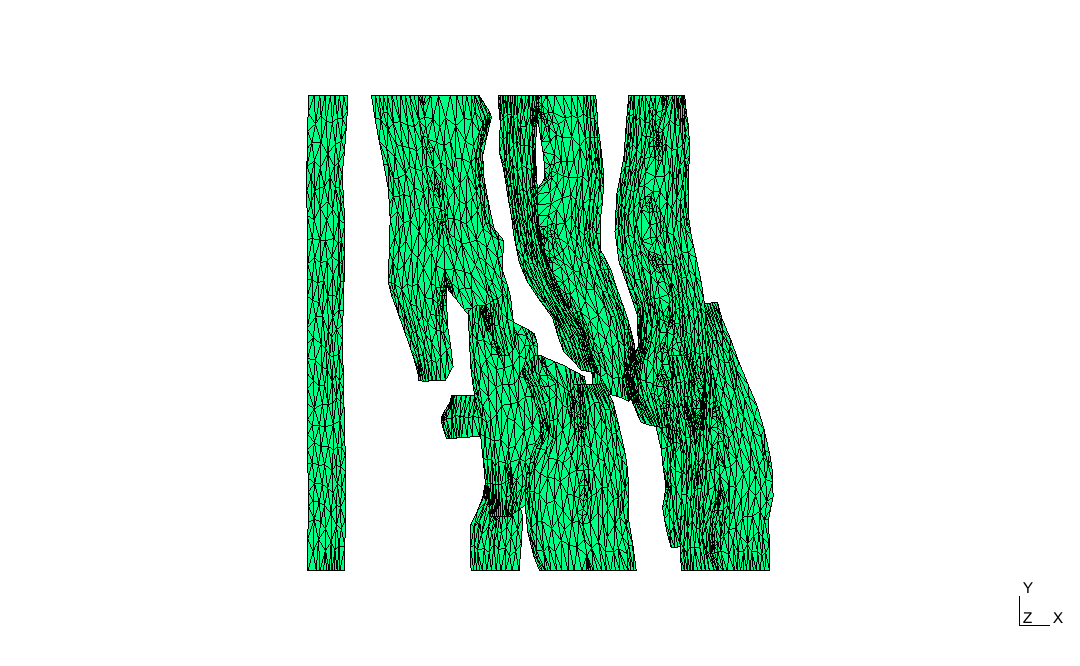
\includegraphics[width=.4\textwidth]{../images/visu_maillage5364FracsTriangles.png}} \quad
\subfloat[][Cluster at the first level.]
   {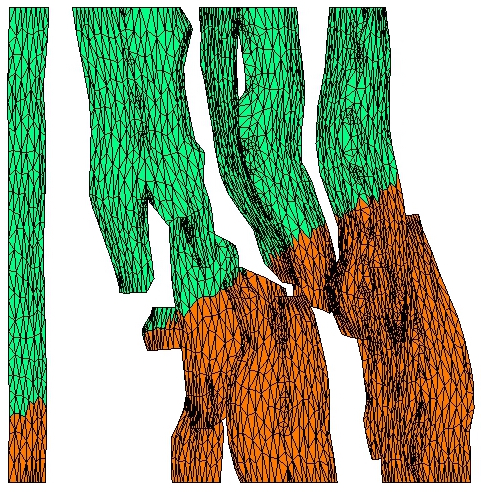
\includegraphics[width=.4\textwidth]{../images/VisuPartmaillage5364FracsTrianglesdepth1.jpg}} \\
\subfloat[][Cluster at the second level.]
   {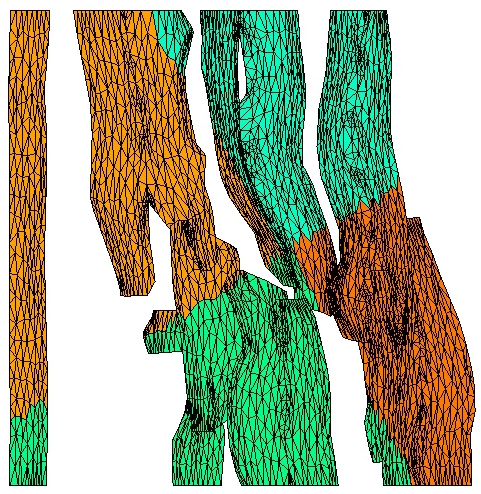
\includegraphics[width=.4\textwidth]{../images/VisuPartmaillage5364FracsTrianglesdepth2.jpg}}  \quad
\subfloat[][Cluster at the third level.]
   {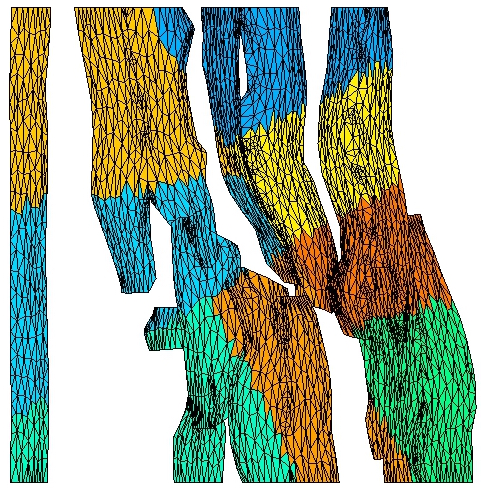
\includegraphics[width=.4\textwidth]{../images/VisuPartmaillage5364FracsTrianglesdepth3.jpg}} \\
\caption{Cluster tree for a fault network.}
\label{fig:cluster_tree_faults}
\end{figure}

\quad\\
To build a subset $\mathscr{B} \in \llbr 1,3N \rrbr \times \llbr 1,3N\rrbr $ of admissible blocks, we can look at pairs of clusters at the same level in the cluster tree and check if they are admissible, starting from the root. If they are, we apply ACA to the corresponding sub-matrix, and if they are not, we look at the interactions between their sons. This recursive algorithm provides a block decomposition like (\ref{eq:decomposition}).
Actually if the block is admissible, we also check if the compression for the given $\varepsilon$ is advantageous in terms of complexity. More precisely, during the algorithm ACA, if $k(n+m)/(n\cdot m) \geq 1$ for a block $n\times m$ and $k$ the current rank of the approximation, we stop and we do like if the block was not admissible because it is not worth compressing it.





